\chapter{Quantum dot characterization with Paraview}

To analyze the charge carrier confinement within the device, the simulation results were processed using Paraview. The following sections describe the charge density distribution and the resulting potential landscape.

\section{Charge density distribution map}
The distribution of the charge density was visualized by performing a \textit{Slice} operation on the 3D model. The slice was taken with a normal vector along the \textbf{Z-direction} at the coordinate \textbf{z = 45}, which corresponds to the active region of the SiMOS structure where the dots are formed.
\begin{figure}[h]
    \centering
    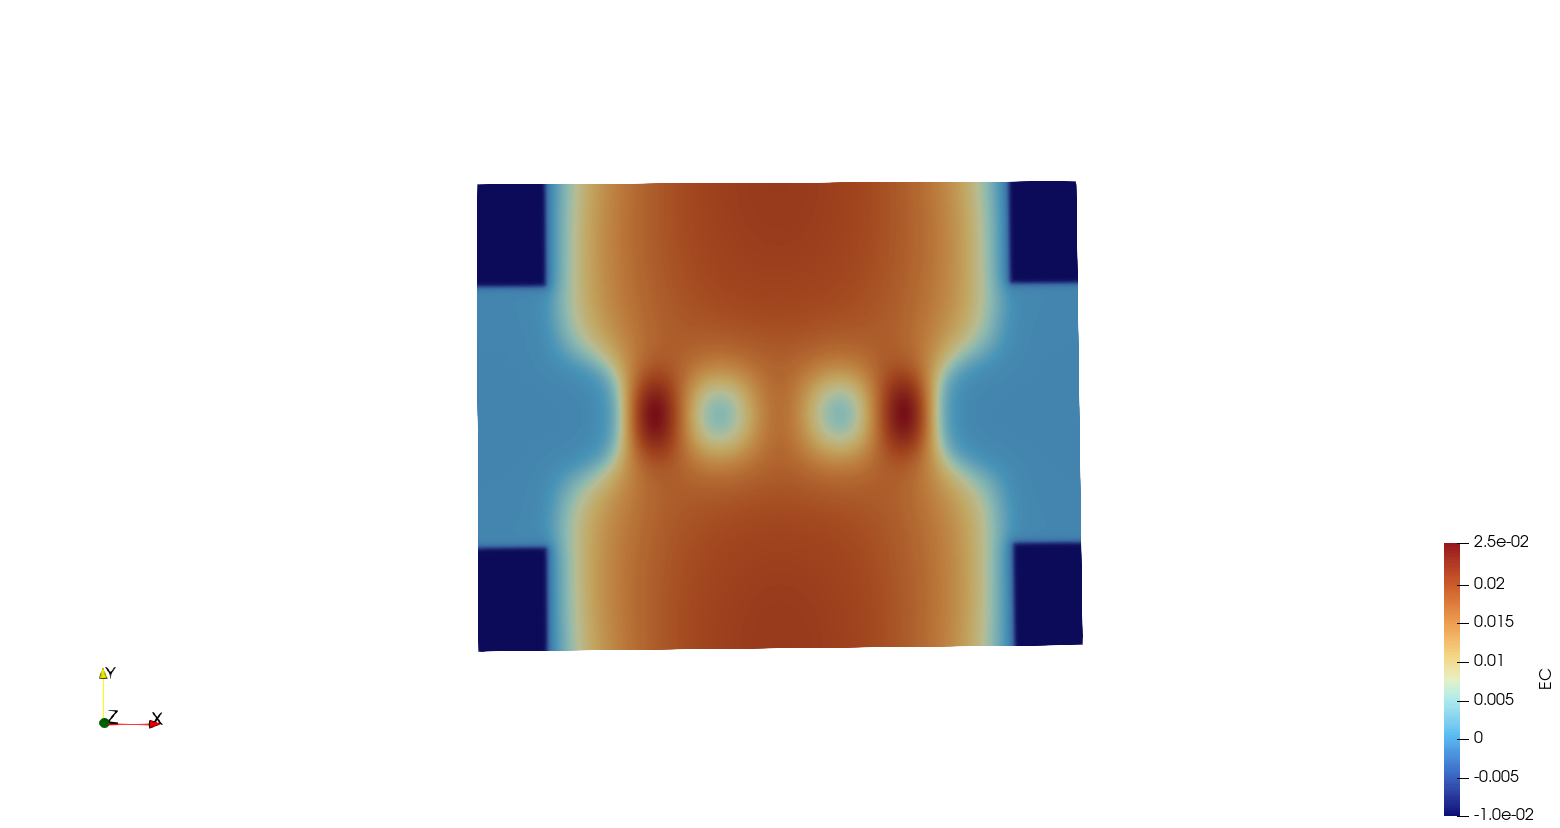
\includegraphics[width=0.7\textwidth]{Images/EC45Z.png}
    \caption{Density charge map (Slice at $z=45$) showing the double quantum dot region.}
    \label{fig:charge_density_map}
\end{figure}

The map in Figure \ref{fig:charge_density_map} illustrates the spatial arrangement of the carriers. The regions characterized by a high concentration of charges are represented in \textbf{dark blue}, which corresponds to the reservoirs and the interior of the dots. Conversely, the areas in \textbf{intense red} represent a very low charge distribution, indicating the presence of electrostatic potential barriers that provide the necessary confinement. In the central area, two distinct charge accumulation zones are visible, identifying the double quantum dot system.

\section{Potential profile analysis}
To further investigate the confinement, a \textit{Plot Over Line} was performed across the domain along the x-axis, at the fixed coordinates $y = 136.5$ and $z = 45$. This profile provides a quantitative view of the potential landscape through the centers of the two dots.

\begin{figure}[h]
    \centering
    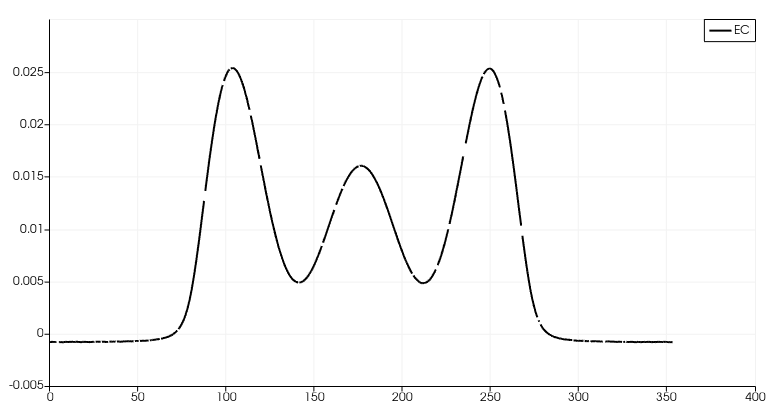
\includegraphics[width=0.7\textwidth]{Images/ECPlot.png}
    \caption{Potential graph (EC) along the x-axis.}
    \label{fig:potential_plot}
\end{figure}

The resulting graph in Figure \ref{fig:potential_plot} confirms the formation of the double quantum dot. However, contrary to our previous laboratory observations, the central potential barrier between the two dots appears significantly lower than, or comparable to, the outer confinement barriers separating the dots from the reservoirs. This behavior, resulting from the specific gate bias configuration applied in the SiMOS device simulation, suggests a different coupling regime between the two quantum dots in this specific instance